\chapter{Classicality in the prepare-and-measure scenario}
\label{chap:pam-classical}

    A key objective in the study of quantum correlations is understanding what makes some behaviors be surely quantum, while others may be not. Progress on this issue improves our understanding of what is ``quantum'' in quantum theory, which in turn will lead to improved or even innovative technological applications.

    In this chapter, I introduce novel methods for deciding whether some set of quantum preparations or quantum measurements behaves classically. These will, in turn, provide new insights about a nonclassicality activation phenomenon and the relation between measurement incompatibility and quantum behaviors in prepare-and-measure scenarios.

    These results were published in \cite{degois_2021_general}, and computational details are provided in appendix \ref{ap:a}.

    \ornamentbreak

    To make the problem we want to solve precise, let us first recall that  the most general prepare-and-measure behaviors involving strictly classical variables are those in $\mathcal{C}^\lambda_{d,B,X,Y}$ (eq.~\eqref{eq:pam-classical-sr}).  Contrastingly, the $\mathcal{Q}_{d,B,X,Y}$ contain the \emph{least} general quantum behaviors, which are those needing only quantum preparations with independent devices (sec. \ref{sec:quantum-behaviors}). The relation $\mathcal{C}_{d,B,X,Y}^\lambda \subset \mathcal{Q}_{d,B,X,Y}$  reflects the fact that some behaviors arising from quantum preparations are nevertheless in $\mathcal{C}_{d,B,X,Y}^\lambda$, while others are definitely not. Those which are, can be simulated by classical preparations with shared randomness. Hereafter, we will call any behavior in the $\mathcal{C}^\lambda_{d,B,X,Y}$ \emph{classically reproducible/simulatable} --- or just \emph{classical}, for short.

    It is important to keep in mind that several distinct notions of classicality exist in the literature. As is the case of entanglement measures, some applications may call for a classicality model or another. Our choice of $\mathcal{C}_{d,B,X,Y}^\lambda$ for the classical behaviors set is general in the sense discussed in chap. \ref{chap:pam}. It is also in line with widely studied classicality models in different correlation scenarios, such as local hidden variables and local hidden states models \cite{brunner_2014_nonlocality,uola_2020_steering,cavalcanti_2016_steering}.

    Suppose a behavior $\mathbf{p}$ arose from a set $\mathcal{S}$ of quantum preparations under some collection of measurements, and furthermore that it is classically reproducible with \emph{d}its. This means that $\mathbf{p} \in \mathcal{C}_{d,B,X,Y}^\lambda$. But it does \emph{not} mean that $\mathcal{S}$ always behaves classically, for it may be the case that different measurements would reveal nonclassicalities in $\mathcal{S}$. Even if we certify $\mathcal{S}$ is classical for all possible sets of $Y$ measurements, it could happen that increasing the number of measurement choices leads to nonclassicality \cite{poderini_pamcriteria_2020}. To better understand what makes quantum preparations behave classically of not, we must then deal with any number of uncharacterized measurements. This is precisely the task we partially solve in sec. \ref{sec:preparation-classicality}. %Certifying that $\mathcal{S}$ is classical for unbounded $Y$ (i.e., irrespective of which and how many measurements Bob may employ) is precisely the task we aim to solve in sec. \ref{sec:preparation-classicality}.

    Before tackling that, it is both instructive and useful to further examine the $\mathbf{p} \in \mathcal{C}_{d,B,X,Y}^\lambda$ membership problem. As previously discussed, any $\mathcal{C}_{d,B,X,Y}^\lambda$ is a polytope, thus set membership can be certified through compliance with a finite set of linear inequalities representing its facets. If one is given the facets, this a computationally easy problem, but obtaining the facets is not. The whole complexity of the problem then lies in characterizing a the polytope for a given scenario. As first noticed in \cite{gallego_pam_2010}, this can be done by enumerating all of $\mathcal{C}_{d,B,X,Y}^\lambda$'s extremal points and finding their convex hull (see sec. \ref{sec:convexity}). The extremal points --- also called \emph{deterministic behaviors/strategies} ---, are found from eq.~\eqref{eq:pam-classical-independent} when the response functions are deterministic, and their enumeration can be cast as the following procedure.

    Let $\mathbf{p}_D = \left( p(b \mid x, y) \right)_{b, x, y}$ be an ordered list representing a deterministic behavior. To simplify the notation, let us consider $b \in \{ 0, 1\}$ (the generalization is straightforward) and write $\mathbf{p}_D = \left( \mathbf{v}_x \right)_{x=1}^X$, where $\mathbf{v}_x = \left( p(b = 0 \mid x, 1), \ldots, p(b = 0 \mid x, Y ) \right)$ will be called a \emph{substring}. Only the $b=0$ probabilities must be considered, as $p(1 \mid x, y) = 1 - p(0 \mid x, y)$. A deterministic behavior is valued as $1$ for one of the outcomes and, of course, $0$ for all others. Whenever $d = X$, there will be $2^{XY}$ distinct $\mathbf{p}_D$ vectors. In this $B=2$ case, those are exactly all possible $XY$-length $d$itstrings but, in the general case, there will be $B^{XY}$ vectors corresponding to only those $(B-1)XY$-length $d$itstrings with a single $1$ in each $B-1$-length consecutive substring. We can think of each of these vectors as a deterministic strategy where Alice's choice of $x$ is unambiguously encoded in a classical state $\tau_x$, from which Bob may then perfectly recover $x$ through classical post-processing. The nontrivial case happens when $d < X$, i.e., when there are only $d$ distinct classical preparations. As the preparation box has more buttons than distinct classical states, at least $\lceil X/d \rceil$ inputs will be mapped to the same message. Whenever $\tau_i = \tau_j$, obviously $\mathbf{v}_i = \mathbf{v}_j$, hence our vector $\mathbf{p}_D$ will have $d - X$ repeated substrings. With this in mind, enumerating all possible deterministic points amounts to generating every unique $dY$-length ditstrings, then repeating $d-X$ substrings $\mathbf{v}_x$ in all possible arrangements.

    The number of deterministic points scales exponentially as $N_\lambda \propto (B-1)^{dY}$, which makes the change to the hyperplane description intractable for all but the smallest parameters. One solvable case that will be used in sec. \ref{sec:nonclassicality-activation} is for $\mathcal{C}^\lambda_{2,2,4,2}$, where the polytope is defined by the two following classes of nontrivial inequalities \cite{poderini_pamcriteria_2020}
    %
    \begin{subequations}
        \begin{gather}
            S = E_{11} - E_{12} - E_{21} + E_{22} - E_{31} - E_{32} + E_{41} + E_{42} \leq 4 \label{eq:inequality-s}\\
            S^\prime = E_{11} + E_{12} + E_{21} - E_{22} - E_{41} \leq 3 
        \end{gather}
    \end{subequations}
    %
    where the $E_{xy}=\condprob{b=0}{x,y}-\condprob{b=1}{x,y}$ are the so-called \emph{correlators}.

    Framing it with quantum preparations, this scenario corresponds to a set $\mathcal{S}$ with $X=4$ possible $d=2$-dimensional quantum systems (qubits) that will be prepared by Alice's device then measured by Bob's. He will have $Y=2$ choices of POVMs, where each POVM is composed of $B=2$ effects. An interesting fact in this scenario (as well as many others) is that some quantum preparations and measurements, even with independent devices, can violate inequalities $S$ or $S^\prime$. When this happens, the behavior is not classically reproducible. In many cases, nonclassicalities provide quantum advantage in informational protocols (sec. \ref{sec:communication-protocols}). 

    %%%%%%%%%%%%%%%%%%%%%%%%%%%%%%%%
    \section{Classicality of preparations}
    \label{sec:preparation-classicality}

        But we are interested in a much more general question than that of certifying whether or not a \emph{behavior} is classically reproducible, namely, that of certifying if the set $\mathcal{S}$ of quantum preparations is itself classical. For that to be true, there must be no measurements that upon acting on $\mathcal{S}$ end up in a nonclassical behavior. Brute-forcing our way into the answer is off the table, for this would amount to testing the behaviors of $\mathcal{S}$ for \emph{all} (infinitely many) possible measurements.

        This is a similar problem to that of finding local hidden variable models for entangled states in Bell scenarios \cite{acin_2006_grothendieck,hirsch_2017_betterlocalhidden}, for which a general computational method guaranteeing a sufficient condition has recently been proposed \cite{cavalcanti_generalmethod_2016,hirsch_algorithmic_2016}. We now adapt it to the prepare-and-measure scenario.

        Suppose that, for the quantum states in $\mathcal{S}$ and a finite set $\mathcal{M} = \{ E_{b \mid y} \}_{b,y}$ of $Y$ measurements, the classical model~\eqref{eq:pam-classical-sr} exists, i.e., that
        %
        \begin{equation}
            \tr{\rho_x E_{b\mid y}} = \int_{\Lambda} \sum_{m = 1}^{d} \pi(\lambda) \condprob{m}{x,\lambda} \condprob{b}{m,y,\lambda} d\lambda \quad\forall b,x,y .
        \label{eq:quantum-classicality-model}
        \end{equation}
        %
        From trace's linearity, for any convex sum of effects,
        %
        \begin{equation*}
            \trb{\rho_x \left( w E_{b\mid y} + (1-w) E_{b^\prime \mid y^\prime} \right)} = w\tr{\rho_x E_{b\mid y}} + (1-w) \tr{\rho_x E_{b^\prime \mid y^\prime}} .
        \end{equation*}
        %
        Whence, $\mathcal{S}$'s behaviors are classical under all measurements in $\conv{\mathcal{M}}$, and in particular for all measurements whose effects are inside the largest ball we can inscribe in $\conv{\mathcal{M}}$ (fig. \ref{fig:measurements-hull}). For normalized Bloch vectors (c.f. eq.~\eqref{eq:normalized-bloch-vector-representation}), $0 \leq \eta \leq 1$ will be its radius. This ball is nothing but a depolarized Bloch ball $\eta \, \blochballd{d}$. This suggests that by probing the preparations with but a finite number of measurements and (possibly) finding a classical model, we can nevertheless certify classicality for the infinitely many measurements whose effects are in $\eta \, \blochballd{d}$. They can be written as
        %
        \begin{equation}
            \Phi_\eta(E_{b \mid y}) = \eta E_{b \mid y} + (1 - \eta) \frac{ \tr{E_{b \mid y}} }{d} \id \equiv E_{b \mid y}^\eta,
            \label{depolarized-measurements}
        \end{equation}
        %
        but they are still not all possible measurements. As an example, unless $\eta = 1$, many rank-1 projective measurements (those on the Bloch sphere) will be left out.

		\begin{figure}
		%
			\begin{minipage}[c]{0.42\textwidth}
				\centering
            	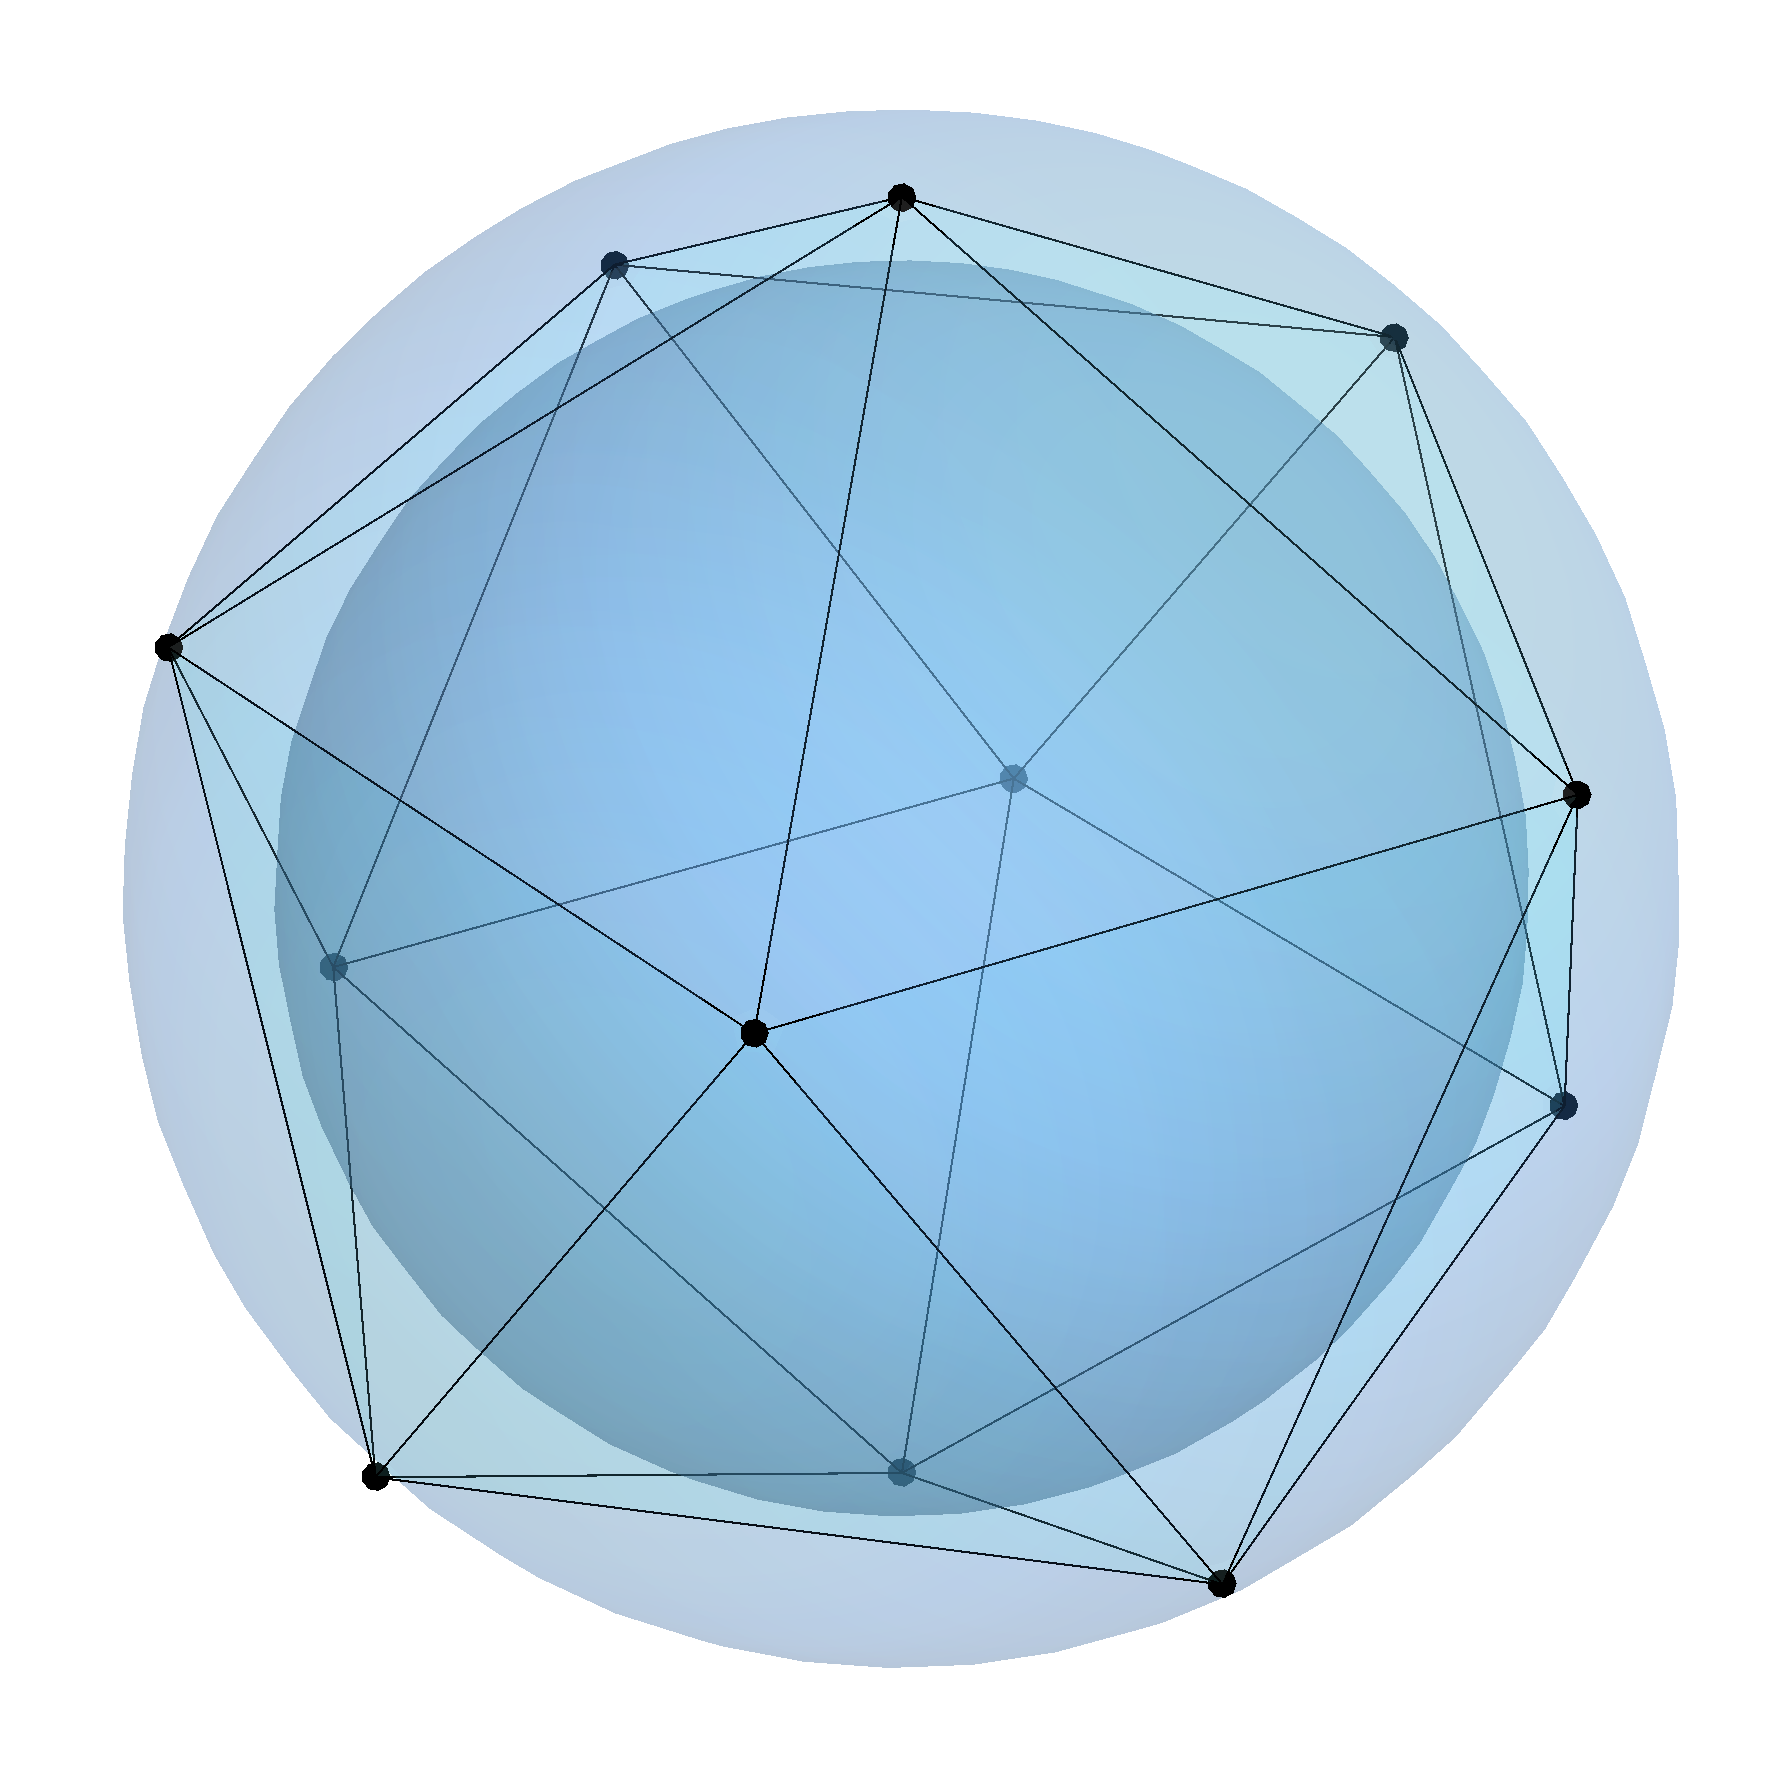
\includegraphics[width=.9\columnwidth]{measurements-hull.png}
			\end{minipage}
			%
			\begin{minipage}[c]{0.56\textwidth}
            	\caption{Representation of the method for $d = 2$. Each vertex on the Bloch sphere represents a measurement operator. To every $\Pi_{0 \vert y}$ we associate a corresponding antipodal $\Pi_{1 \vert y}$. Measurements inside the set enclosed by $\textbf{conv}(\mathcal{M})$ can be simulated by mixing these extremal ones. In particular, any measurement $\{ \Pi_{b \vert u}^\eta \}_b$ in a ball with radius $\eta$ inscribed in the polytope is simulable in such manner.}
   		    	\label{fig:measurements-hull}
			\end{minipage}
		\end{figure}

        The work-around is to consider the dual map $\Phi_\eta^\dagger$ applied to the preparations. This will result in each
        %
        \begin{equation}
            \rho_x \mapsto \Phi_\eta^\dagger(\rho_x) = \frac{1}{\eta} \left[ \rho_x - (1 - \eta) \frac{\id}{d} \right] \equiv O_x .
            \label{eq:polarized-preparations}
        \end{equation}
        %
        Analyzing the behavior of the $O_x$ under the $E_{b \mid y}^\eta$ tells us that
        %
        \begin{align*}
            \tr{O_x E_{b \mid y}^\eta} &= \text{tr}\left\{ \frac{1}{\eta} \left[ \rho_x - (1 - \eta) \frac{\mathbf{1}}{d} \right]  \left[ \eta E_{b \mid y} + (1 - \eta) \frac{ \tr{E_{b \mid y}} }{d} \id \right] \right\} \\
            &= \tr{\rho_x E_{b \mid y}} - \left[ \frac{1 - \eta}{d} - \frac{ 1 - \eta }{ d \eta }  + \frac{ (1 - \eta)^2 }{ d \eta } \right] \tr{E_{b \mid y}}.
        \end{align*}
        %
        If all effects $E_{b \mid y}$ are rank-1 projectors, then $\tr{E_{b \mid y}} = 1$ (sec. \ref{sec:gell-mann}), making it true that
        %
        \begin{equation}
            \tr{O_x E_{b \mid y}^\eta} = \tr{\rho_x E_{b \mid y}}.
            \label{eq:trace-equality-preparation-classicality}
        \end{equation}

        The procedure to test $\mathcal{S}$ for classicality follows from precisely this trace equality relation. We start out by defining an operator $O_x$ for each state $\rho_x \in \mathcal{S}$. Ensuingly, we probe the $\mathcal{O} = \{ O_x \}_x$ with some set $\mathcal{M} = \{ E_{b \mid y} \}_{b,y}$ of rank-1 projective measurements. If the model on the r.h.s. of eq.~\eqref{eq:quantum-classicality-model} exists for $\mathcal{O}$ and $\mathcal{M}$, the preceding discussion reveals it also exists for every measurement in $\conv{\mathcal{M}}$. It will then be true that $\mathbf{p} = \Big\{ \tr{O_x E_{b \mid y}^\eta} \Big\}_{b,x,y}$ is a classical behavior for \emph{all} measurements whose effects can be written as $E_{b \mid y}^\eta$. In turn, eq.~\eqref{eq:trace-equality-preparation-classicality} implies that the $\rho_x$ admit a classical model for all $E_{b \mid y}$, which are all rank-1 projections. Measurement results for projections of larger rank can be inferred from rank-1 projections through coarse graining (classical post-processing), hence the result is valid for all projective measurements.

        To cast this procedure as an optimization problem, recall that the deterministic strategies $\lambda$ can be enumerated as discussed in the previous section. Assuming that is done, the integral in~\eqref{eq:quantum-classicality-model} turns into a finite sum. Besides, the distance from the nearest hyperplane in the convex hull of $\mathcal{M}$ to the origin is $\eta$. Further observing that the maximally mixed state $\id/d$ is trivially classical, we write
        %
        \begin{subequations}
            \begin{alignat}{2}
                &\text{given}    &\quad & \mathcal{S},\, \mathcal{M},\, \eta, \{ \lambda \} \\
                &\underset{\pi(\lambda)}{\text{max.}}   &	  & \alpha \\
                &\text{s.t.}    &      & \alpha \rho_x + (1 - \alpha)\frac{\mathbf{1}}{d} = \eta O_x + \left( 1 - \eta \right) \frac{\mathbf{1}}{d}, \quad\forall x \label{eq:cond-1}\\
                &                  &      & \text{tr}(E_{b \vert y} O_x) = \sum_{m, \lambda} \pi(\lambda) p(m \vert x, \lambda) p(b \vert m, y, \lambda), \quad\forall b, x, y \label{eq:cond-2}\\
                &				   &	  & 0 \leq \alpha \leq 1 \\
                &				   &	  & \pi(\lambda) \geq 0 \\
                &				   &	  & \sum_\lambda \pi(\lambda) = 1 \label{eq:cond-5}.
            \end{alignat}
            \label{eq:preparation-classicality-projective}
        \end{subequations}
        %        
        Allowing the $\rho_x$ to be mixed with the identity in the l.h.s. of eq.~\eqref{eq:cond-1} guarantees the program will always have a feasible solution. Constraints \eqref{eq:cond-2}--\eqref{eq:cond-5} force the local model to exist, the mixtures to be valid density operators, and $\pi$ to be a probability distribution over the deterministic strategies, respectively. Any solution where $\alpha = 1$ certifies that preparations in $\mathcal{S}$ admit a classical model for all projective measurements. On the other hand, any $\alpha < 1$ certifies only that the preparations $\alpha \mathcal{S} = \{ \alpha \rho_x \}_x$ are classical. This criterion turns from sufficient to both necessary and sufficient only when $\eta \rightarrow 1$, a regime approachable by increasing the number $Y$ of probe measurements.

        Being a linear program (sec. \ref{sec:linear-programming}), eq.~\ref{eq:preparation-classicality-projective} can be efficiently solved up to numerical precision. Regardless of linear programming complexity, an instance of program~\eqref{eq:preparation-classicality-projective} has $N_\lambda$ variables. As already noted, $N_\lambda \propto (B-1)^{dY}$ thus the program size scales exponentially with the number of measurements. It will always be of interest to maximize $\eta$, and consequently, to maximize $Y$. With $X=4$ preparations, a common desktop computer can usually only handle less than $Y = 12$ projective qubit measurements. This limitation can be circumvented through the iterative optimization procedure described in sec. \ref{ap:a-computational}, which was applied in all upcoming results.

        It is also possible to extend our criterion to non-projective measurements. Dichotomic projective measurements are the extremal two-outcome POVMs. Consequently, out method actually guarantees classicality for all $B=2$-outcome measurements. For all other cases, we can extend it by simulatating POVMs with projective measurements (c.f. sec. \ref{sec:measurements}). To see how, recall that any set of generalized measurements $\mathcal{M} = \{ E_{b \mid y} \}_{b,y}$ becomes projective-simulatable after a certain amount $t$ of depolarization Observing that
        %
        \begin{equation}
            \trb{E_{b \mid y} \Phi_t(\rho_x)} = \trb{\Phi_t(E_{b \mid y}) \rho_x}
        \end{equation}
        %
        leads us to conclude that testing $\mathcal{S} = \{ \rho_x \}_x$ for classicality under all POVMs is the same as certifying that preparations
        %
        \begin{equation}
            \rho^\prime_x \equiv \Phi_t^\dagger \left( \rho_x \right) = \frac{1}{t} \left( \rho_x - \frac{1-t}{d} \id \right)
        \end{equation}
        %
        are classical for all projective measurements, where $t$ is some amount of depolarization such that $\Phi_t(\mathcal{M})$ are projective-simulatable.

        Program~\eqref{eq:preparation-classicality-projective} can be easily modified to this case by either adding an extra constraint or through explicit rewriting. For the former, it reads
        %
        \begin{subequations}
            \begin{alignat}{2}
                &\text{given}    &\quad & \mathcal{S},\, \mathcal{M},\, \eta, \{ \lambda \}, t \\
                &\underset{\pi(\lambda)}{\text{max.}}   &	  & \alpha \\
                &\text{s.t.}    &      & \rho_x^\prime = \frac{1}{t} \left( \rho_x - \frac{1-t}{d} \id \right), \quad\forall x \\
                &               &      & \alpha \rho_x^\prime + (1 - \alpha)\frac{\mathbf{1}}{d} = \eta O_x + \left( 1 - \eta \right) \frac{\mathbf{1}}{d}, \quad\forall x \\
                &                  &      & \text{tr}(E_{b \vert y} O_x) = \sum_{m, \lambda} \pi(\lambda) p(m \vert x, \lambda) p(b \vert m, y, \lambda), \quad\forall b, x, y \\
                &				   &	  & 0 \leq \alpha \leq 1 \\
                &				   &	  & \pi(\lambda) \geq 0 \\
                &				   &	  & \sum_\lambda \pi(\lambda) = 1 ,
            \end{alignat}
            \label{eq:preparation-classicality-povm}
        \end{subequations}
        % 
        which is also a linear program.


        %%%%%%%%%%%%%%%%%%%%%%%%%%%%%%%%%%%%%%%%%%%
        \subsection{Nonclassicality activation and quantum advantage in a RAC}
        \label{sec:nonclassicality-activation}

            Nonclassicality activation phenomena have been long-known in Bell scenarios, where an entangled state that only behaves locally may have its nonlocality activated, for instance, by local filtering, broadcasting, or by exploring multiple copies of the state \cite{popescu-filtering-1995, hirsch-hidden-2013,gallego2014nonlocality,navascues-activation-2011, palazuelos-superactivation-2012,cavalcanti2011quantum,bowles2020singlecopy}. Very recently, two interesting, similar phenomena were explored in PM scenarios \cite{poderini_pamcriteria_2020} --- one related to increasing the number of allowed measurements, and the other to the number of preparations. Our method can be applied to demonstrate a stronger form of the latter.

            Let us start by defining $\mathcal{S}(\alpha, \theta) = \{ \rho_{\mathbf{r_1}}, \rho_{\mathbf{r_2}}, \rho_{\mathbf{r_3}}, \rho_{\mathbf{r_4}} \}$ as the preparation set illustrated in fig. \ref{fig:preparation-set-activation}. They are parametrized by $\alpha$ --- a shrinking factor from the surface of the Bloch sphere ---, and the angle $\theta$. For the probe measurements, we will choose the ones parametrized by the Bloch vectors $\mathbf{q}_1 = (- \mathbf{x} + \mathbf{z}) / \sqrt{2}$ and  $\mathbf{q}_2 = (\mathbf{x} + \mathbf{z}) / \sqrt{2}$. Substituting back into inequality $S$ (eq.~\eqref{eq:inequality-s}), we get that $S(\alpha, \theta) = 4\sqrt{2} \alpha \sin \theta$. This curve is shown in fig. \ref{fig:nonclassicality-activation}, where any violation of $S \leq 4$ certifies nonclassicality.

            Our second step is to take every subset of $3$ preparations from $\mathcal{S}(\alpha, \theta)$ at some $\theta$. For each possibility, we run program~\eqref{eq:preparation-classicality-projective} and find the largest $\alpha^*$ such that \emph{any} collection of $3$ preparations is classical. Any $\alpha < \alpha^*$ has more of the identity state, thus preserves classicality. Sweeping $\theta$, we obtain the dotted curve shown in fig. \ref{fig:nonclassicality-activation}. The shaded region then corresponds to a situation where all triads of preparations are classical, but that taken together have their nonclassicality activated.

			\begin{figure*}[t!]
				\newdimen\subfigcapmargin  \subfigcapmargin  =  -3em
				\centering
				%
				\subfigure[Preparations]{\label{fig:preparation-set-activation}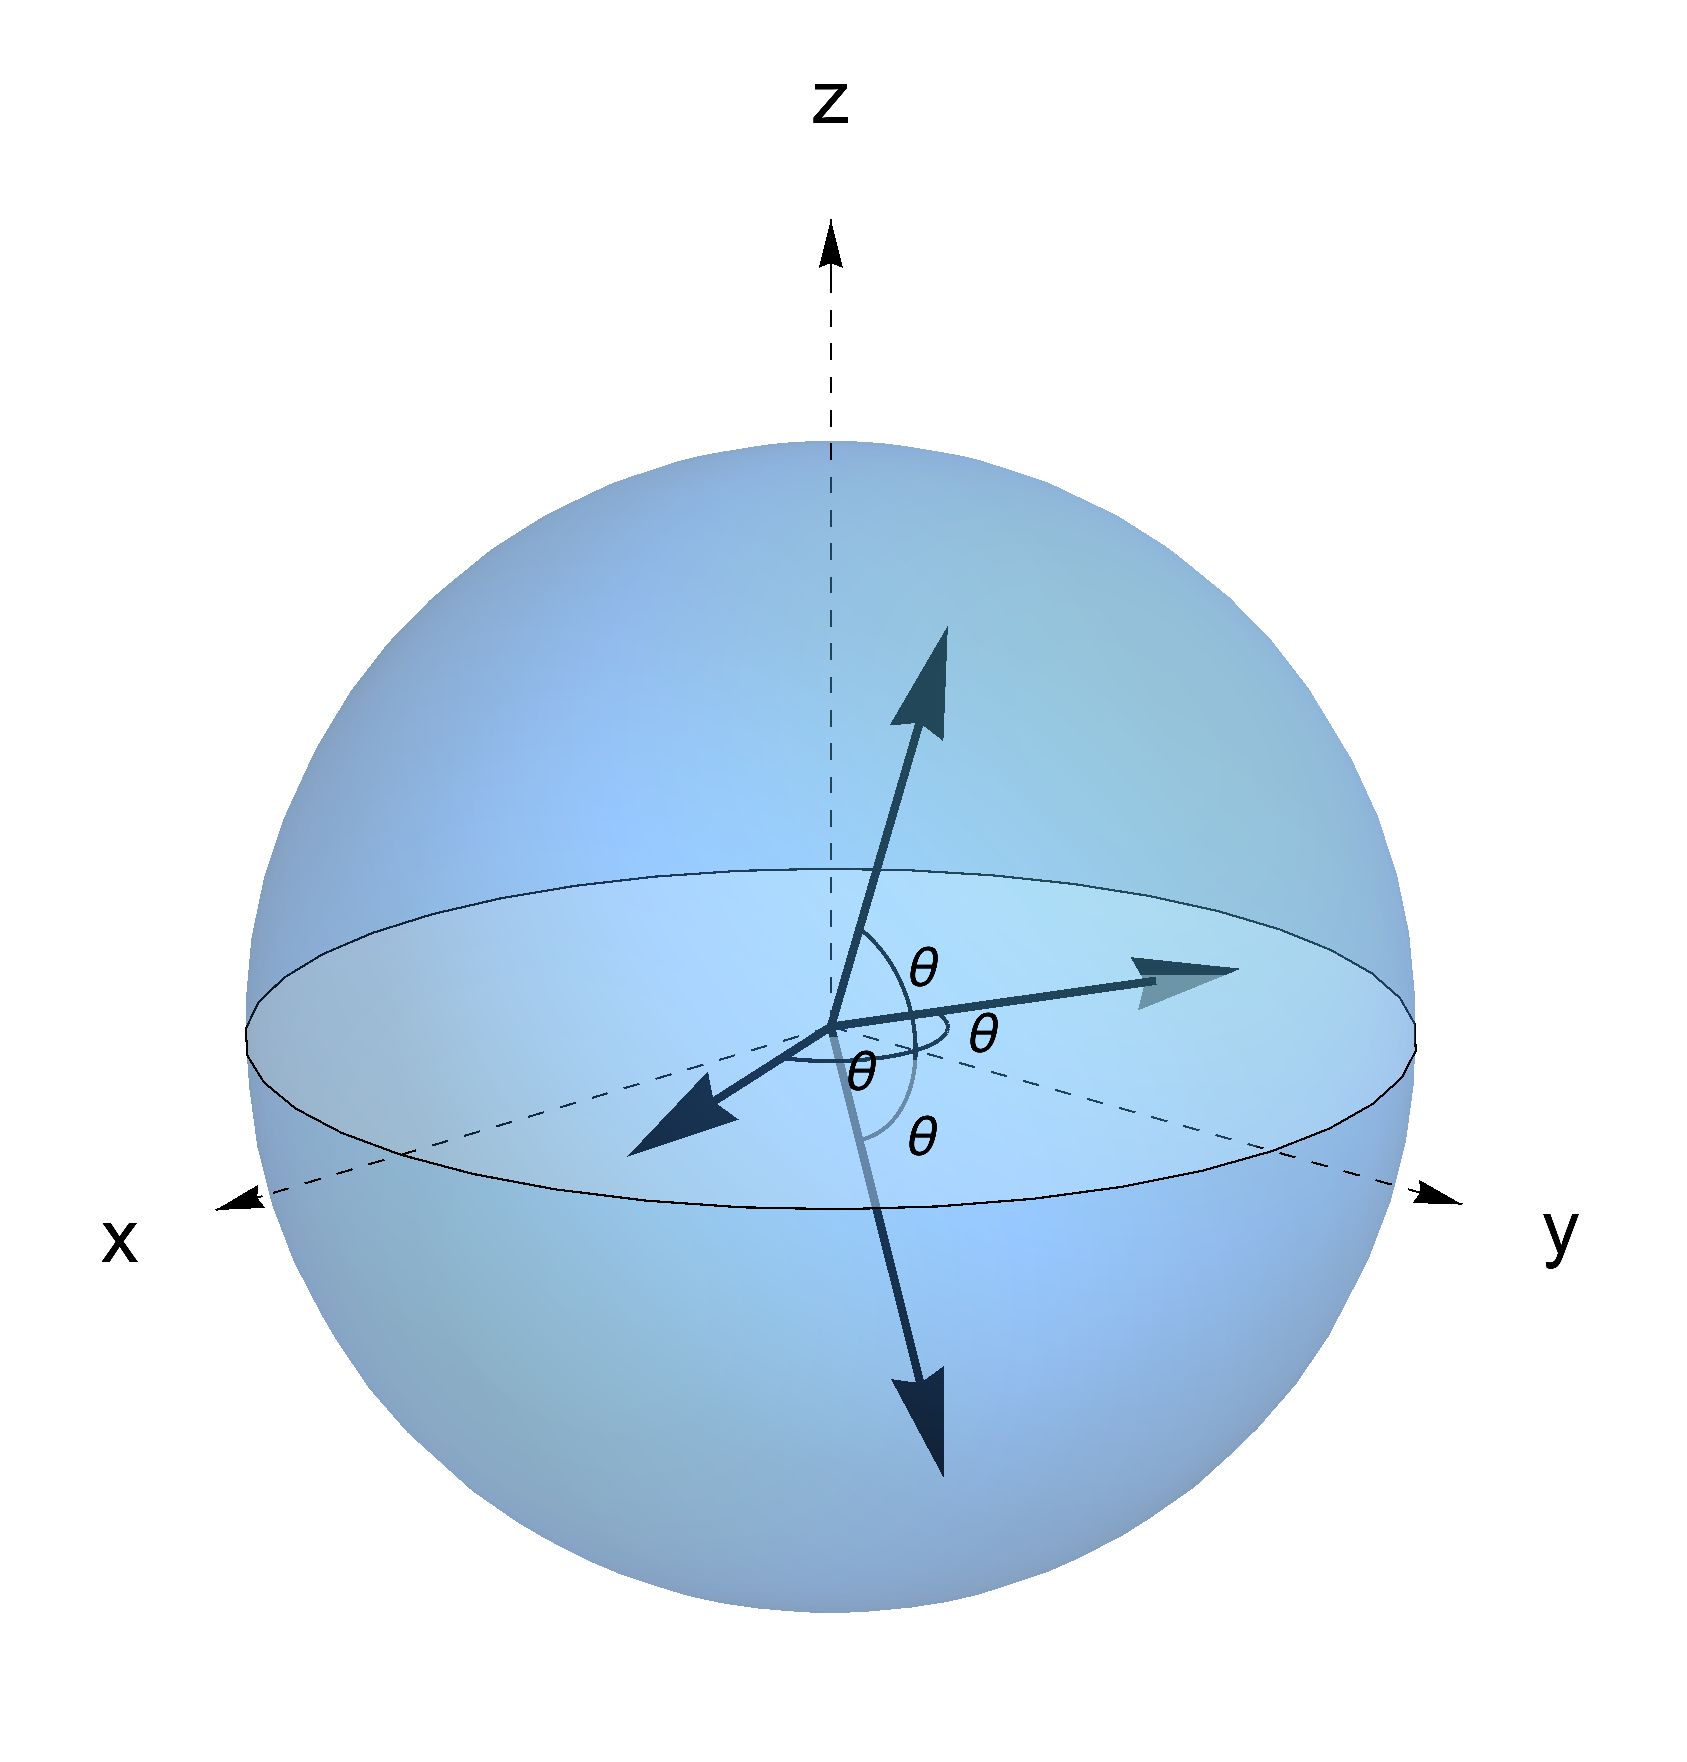
\includegraphics[width=.4\linewidth]{preparation-states.png}}\hfill
				\subfigure[Activation]{\label{fig:nonclassicality-activation}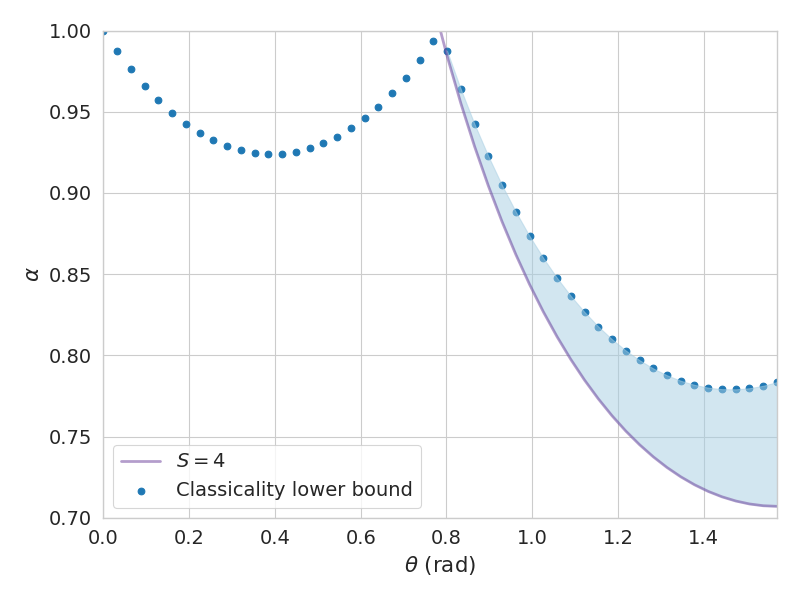
\includegraphics[width=.58\linewidth]{preparation-activation.png}}\hfill
				%
				\caption{Nonclassicality activation in the prepare-and-measure scenario. On the left, preparations $\mathcal{S}(\alpha, \theta) = \{ \rho_{\mathbf{r_1}}, \rho_{\mathbf{r_2}}, \rho_{\mathbf{r_3}}, \rho_{\mathbf{r_4}} \}$ are represented by their Bloch vectors, for $\alpha=0.8$. At $\theta=0$, all preparations are at $\alpha \mathbf{y}$. For $\theta = \pi/2$, $\mathcal{S} =  \{ -\alpha\mathbf{x}, \alpha\mathbf{x}, -\alpha\mathbf{z}, \alpha\mathbf{z} \}$, corresponding to the largest violation of inequality \eqref{eq:inequality-s}. On the right, result of applying program \ref{eq:preparation-classicality-projective} to $\mathcal{S}$. To run it, $12$ probe measurement effects arranged as the vertices of a rhombicuboctahedron ($\eta \approx 0.86$). As $S \propto \alpha$, every preparation set above the $S=4$ curve is non-classical. On the other hand, the classicality curve shows the maximum visibility such that any triad of states in the preparation set are classical. The shaded region thence represents sets of four preparations that are three-wise classical, but that that when taken together behave nonclassically. In this sense, nonclassicality is activated by measurement inclusion.}
			\end{figure*}
            
            The significance of this results can be illustrated when considering a $\rac{2}{2}{1}$ RAC. Section \ref{sec:racs}) tells us it can me mapped to a $(d,B,X,Y) = (2,2,4,2)$ prepare-and-measure instance, which is exactly the case for the class of inequalities represented by $S$. A \emph{class} is a collection of inequalities that are equivalent through symmetries. In correlation scenarios, these symmetries are called \emph{relabelings}. Because the labels attached to outcomes, preparations and measurements are arbitrary, inequalities obtained from another through relabeling $b$, $x$ and/or $y$ are equivalent. In particular, $s = E_{11} + E_{12} + E_{21} - E_{22} - E_{31} + E_{32} - E_{41} - E_{42} \leq 4$ is a relabeling of $S$. Borrowing from \cite{pawlowski_pamqkd_2011}, we note that, for the $\rac{2}{2}{1}$ RAC, the average probability of success \emph{is} the facet $s$. To see that, let's relabel preparations $\left( 1, 2, 3, 4 \right) \mapsto \left(00, 01, 10, 11\right)$ and open up
            %
            \begin{align*}
                        p_{\text{suc}}^{\text{avg}} &= \frac{1}{8} \sum_{\mathbf{x}, y} p(b = x_y \vert x_0 x_1, y) \\
                        \begin{split}
                            &= \frac{1}{8} \big[ p(0 \vert 00, 0) + p(0 \vert 00, 1) + p(0 \vert 01, 0) + p(1 \vert 01, 1) + \\
                            &\quad\qquad + p(1 \vert 10, 0) + p(0 \vert 10, 1) + p(1 \vert 11, 0) + p(1 \vert 11, 1) \big]
                        \end{split}
                        \\
                        \begin{split}
                            &= \frac{1}{8} \big[ p(0 \vert 00, 0) + p(0 \vert 00, 1) + p(0 \vert 01, 0) - p(0 \vert 01, 1) + \\
                            &\quad\qquad - p(0 \vert 10, 0) + p(0 \vert 10, 1) - p(0 \vert 11, 0) - p(0 \vert 11, 1) + 4 \big]
                        \end{split}
            \end{align*}
            %
            Switching $s$ to full-form and applying normalization, we get
            %
            \begin{align*}
            \begin{split}
                s &= 2 \big[ p(0 \vert 00, 0) + p(0 \vert 00, 1) + p(0 \vert 01, 0) - p(0 \vert 01, 1) + \\
                &\qquad\qquad - p(0 \vert 10, 0) + p(0 \vert 10, 1) - p(0 \vert 11, 0) - p(0 \vert 11, 1) \big] ,
            \end{split}
            \end{align*}
            %
            and together,
            %
            \begin{equation}
                p_{\text{avg}} = \frac{1}{8} \left( \frac{1}{2} s + 4 \right) = \frac{s + 8}{16} \leq \frac{3}{4} ,
                \label{eq:s-vs-pavg}
            \end{equation}
            %
            where the classical bound for $s$ was substituted in the last term. This relation means that any violation of $s$ in the $(2,2,4,2)$ PM scenario can be associated with a quantum advantage in the corresponding $\rac{2}{2}{1}$ QRAC. We have numerically found a lower bound for the maximum quantum violation of $s$ to be approximately $5.65685$. Substituting into eq.~\eqref{eq:s-vs-pavg}, $p_{\text{avg}} \approx 0.853553$, exactly matching the result found in sec. 3.3.1. of \cite{ambainis_srqracs_2009}. This also suggests that our bound for $s$ is tight. More interestingly yet, this construction shows that the nonclassicality activation phenomenon reported above also transfers to this case, where it can be interpreted as an activation of quantum advantage in a relevant quantum communication protocol. 


    %%%%%%%%%%%%%%%%%%%%%%%%%%%%%%%%
    \section{Classicality of measurements}
    \label{sec:measurement-classicality}

        In the absence of entanglement, one must look for other quantum features to explain nonclassical behaviors. Measurement incompatibility (sec. \ref{sec:measurements}) is usually at the center of many interesting quantum phenomena, and from a more practical perspective they may be seen as resources in informational tasks \cite{giovannetti_metrology_2006}. It is then natural to wonder whether non-joint measurability is necessary, or even sufficient, for the arisal of classically irreproducible behaviors in the prepare-and-measure scenario. Reframing the question, we ask: given a set of incompatible measurements, is there \emph{always} some set of preparations that leads to nonclassicality?

        The question at hand has been positively answered for quantum steering \cite{quintino_incompatibilitysteering_2014,uola_incompatibilitysteering_2014,uola_onetoonesteering_2015} and negatively for Bell nonlocality \cite{quintino_2016_incompatibilitybell,quintino_2018_incompatibilitybellgeneral,bene_2018_incompatibilitybell}, but only partial results exist for prepare-and-measure scenarios \cite{carmeli_racsincompatibility_2020}. Interestingly, this problem is similar to what we have just dealt with, but while we were previously interested in certifying some set of preparations is classical for all measurements, we now move on to certify there exists no set of \emph{preparations} such that a fixed set of measurements unveils nonclassicality. We will soon see the previous method is straightforwardly adaptable. Even so, regarding the existing literature, this is a more innovative approach. While Sec. \ref{sec:preparation-classicality} develops a procedure akin to known results for different correlation scenarios \cite{cavalcanti_generalmethod_2016,hirsch_algorithmic_2016}, the method we now present has not, to the best of my knowledge, been considered elsewhere.

        \ornamentbreak

        Starting with the measurement set $\mathcal{M} = \{ E_{b \mid y} \}_{b,y}$ of our interest, we build the operators
        %
        \begin{equation}
            O_{b \mid y} = \eta E_{b \mid y} + (1 - \eta)\frac{\tr{E_{b \mid y}}}{d} \id ,
        \label{eq:polarized-measurements}
        \end{equation}
        %
        where $\eta$ will soon be defined. For some set $\mathcal{S} = \{ \rho_x \}_x$ of \emph{pure} probe preparations, we consider the behavior $\mathbf{p} = \{ \tr{O_{b \mid y} \rho_x } \}$. If, for all $b$, $x$ and $y$, classicality (in the sense of eq.~\eqref{eq:pam-classical-sr}) holds, then it also does for every preparation in $\conv{\mathcal{S}}$. In particular, this will be true for all quantum states in the largest sphere inscribed in the convex hull of $\mathcal{S}$. We write $\eta$ for its radius, and $\rho_x^\eta$ for any preparation in it. A key difference from sec. \ref{sec:preparation-classicality} is that the $\eta$ defining the $O_{b \mid y}$ is now the radius with respect to $\conv{\mathcal{S}}$, as opposed to $\conv{\mathcal{M}}$.

        Our working hypothesis is that
        $$
            \tr{ O_{b \mid y} \rho_x} = \int_{\Lambda} \sum_{m = 1}^{d} \pi(\lambda) \condprob{m}{x,\lambda} \condprob{b}{m,y,\lambda} d\lambda \quad\forall b,x,y .
        $$
        From the discussion in the previous section, this would imply the collection of $\tr{ O_{b \mid y} \rho_x^\eta}$ is also classical for \emph{every} preparation in the $\eta$-sphere. Similarly to the trace equality~\eqref{eq:trace-equality-preparation-classicality}, $\tr{ O_{b \mid y} \rho_x^\eta} = \tr{E_{b \mid y} \rho_x}$ holds whenever the $E_{b \mid y}$ are rank-1 projectors, as can be seen by direct calculation. The r.h.s. of this last equation then tells the measurements in $\mathcal{M}$ leads to classicality for every possible $\rho_x$. Recalling we started with pure preparations, this procedure reveals that such a set of rank-1 projective measurements is classical in regard to all pure states. Pure states are the extremal points in the set of quantum states, thence, any state is a convex combination of those, and the result is valid for all states. Moreover, coarse graining of rank-1 projective measurements simulates PVMs with all larger ranks, proving our procedure works for all projective measurements.

        A slight modification of program~\eqref{eq:preparation-classicality-projective} implements this criterion as the linear program
        %
        \begin{subequations}
            \begin{alignat}{2}
                &\text{given}    &\quad & \mathcal{S},\, \mathcal{M},\, \eta, \{ \lambda \} \\
                &\underset{\pi(\lambda)}{\text{max.}}   &	  & \alpha \\
                &\text{s.t.}    &      & \alpha E_{b \mid y} + (1 - \alpha)\frac{\mathbf{1}_d}{d} = \eta O_{b \mid y} + \left( 1 - \eta \right) \frac{\mathbf{1}_d}{d}, \quad\forall x \\
                &                  &      & \text{tr}(O_{b \vert y} \rho_x) = \sum_{a, \lambda} \pi(\lambda) p(a \vert x, \lambda) p(b \vert a, y, \lambda), \quad\forall b, x, y \\
                &				   &	  & 0 \leq \alpha \leq 1 \\
                &				   &	  & \pi(\lambda) \geq 0 \\
                &				   &	  & \sum_\lambda \pi(\lambda) = 1 .
            \end{alignat}
            \label{eq:measurement-classicality-projective}
        \end{subequations}
        %
        Running it amounts to choosing a suitable set of pure probes $\mathcal{S} = \{ \rho_x \}_x$, finding its corresponding $\eta$, generating the deterministic strategies $\{ \lambda \}$, and querying for the maximum $\alpha$ such that the projective measurements in $\mathcal{M}$ are classical. As before, $\alpha = 1$ certifies they are classical, while $\alpha < 1$ tells us only that the measurements $\mathcal{M}_\alpha = \{ \Phi_\alpha \left( E_{b \mid y} \right) \}_{b,y}$ are. From self-duality of the depolarizing map $\Phi$, another valid interpretation is that $\mathcal{M}$ is classical for all preparations at least as mixed as $\Phi_\alpha \left( \rho_x \right)$.

        Once more in full analogy to the preparation classicality case, we may use concepts of projective simulatability to extend this criterion to POVMs. Let $t$ be a depolarization parameter that turns a POVM set $\mathcal{M}$ projective-simulatable, and recal that $\trb{ \phi_t( E_{b \mid y}) \rho^t } = \trb{ E_{b \mid y} \phi_t(\rho) }$. Testing $\mathcal{M}$ for classicality is hence equivalent to certifying $\Phi_t \left( \mathcal{M} \right)$ is classical with respect to a set
        $$
            \mathcal{S}^t = \{ \rho_x^t \}_x = \Bigg\{ \frac{1}{t} \left( \rho_x - \frac{1-t}{d} \mathbf{1} \right) \Bigg\}_x
        $$
        of probe preparations. Starting from a set $\mathcal{S}$ of pure probes, program~\eqref{eq:measurement-classicality-projective} can be undemandingly modified to implement this criterion, resulting in
        %
        \begin{subequations}
            \begin{alignat}{2}
                &\text{given}    &\quad & \mathcal{S},\, \mathcal{M},\, \eta, \{ \lambda \}, t \\
                &\underset{\pi(\lambda)}{\text{max.}}   &	  & \alpha \\
                &\text{s.t.}    &      & \alpha E_{b \mid y} + (1 - \alpha)\frac{\mathbf{1}_d}{d} = \eta O_{b \mid y} + \left( 1 - \eta \right) \frac{\mathbf{1}_d}{d}, \quad\forall x \\
                &                  &      & \rho_x^\prime = \frac{1}{t} \left( \rho_x - \frac{1-t}{d} \mathbf{1} \right) \\
                &                  &      & \text{tr}(O_{b \vert y} \rho_x^\prime) = \sum_{a, \lambda} \pi(\lambda) p(a \vert x, \lambda) p(b \vert a, y, \lambda), \quad\forall b, x, y \\
                &				   &	  & 0 \leq \alpha \leq 1 \\
                &				   &	  & \pi(\lambda) \geq 0 \\
                &				   &	  & \sum_\lambda \pi(\lambda) = 1 .
            \end{alignat}
            \label{eq:measurement-classicality-povm}
        \end{subequations}
        %
        While, as discussed around program~\eqref{eq:measurement-classicality-projective}, we must start with a set $\mathcal{S}$ of pure probe preparations, there is no issue in working with operators $\rho^t \in \mathcal{S}^t$ inside program~\eqref{eq:measurement-classicality-povm}, as all quantum states are more mixed than those.

        To demonstrate the usefulness of our method, we solve an important question on the relation between measurement incompatibility and classicality in the PM scenario.

        %%%%%%%%%%%%%%%%%%%%%%%%%%%%%%%%%%%%
        \subsection{Measurement incompatibility is insufficient for nonclassicality}
        \label{sec:incompatibility-vs-classicality}

            Non-joint measurability is an important concept of measurement incompatibility with a clear operational interpretation (sec. \ref{sec:measurements}). Withal, incompatibility robustness is an useful measure of the extent to which a set of measurements is non-jointly measurable, and it can be efficiently computed through semidefinite programming (sec. \ref{sec:incompatibility-robustness}). Employing our measurement classicality certification procedure, we now prove measurement incompatibility is insufficient for nonclassicality in prepare-and-measure scenarios.

            Define the $Y=3$ parametrized mirror-symmetric projective measurements defined as shown in fig. \ref{fig:mirror-symmetric-measurements}. For each value of $\theta$, their incompatibility robustness is given by
            %
            \begin{equation}
                    \chi^*_\mathcal{M} = \sup_{\substack{\chi \,\in\, [0, 1]\\ \{ N_{b \mid y}\} \,\in\, \textbf{N}( \mathcal{M} )}} \Big\{ \chi \mid \chi \{ E_{b \mid y} \} + (1 - \chi) \{ N_{b \mid y} \} \in \textbf{JM} \Big\} ,
            \end{equation}
            %
            where $\mathbf{N}(\mathcal{M})$ is a choice of noise model which is generally dependant on the desired application. Unbiased (or white) noise $N_{b|y} = \mathbf{1}/\abs{\mathcal{B}}$ is a common choice when one wants to model experimental imperfections that affect all degrees of freedom undiscriminately. Considering this choice, the lower curve in fig. \ref{fig:incompatibility-vs-classicality} stands for $\chi^*_{\mathcal{M}(\theta)}$, and it is a tight upper bound, up to numerical precision. Consequently, any value of $\chi$ above it defines a non-jointly measurable measurement set.

            % \begin{figure}
            %     \centering
            %     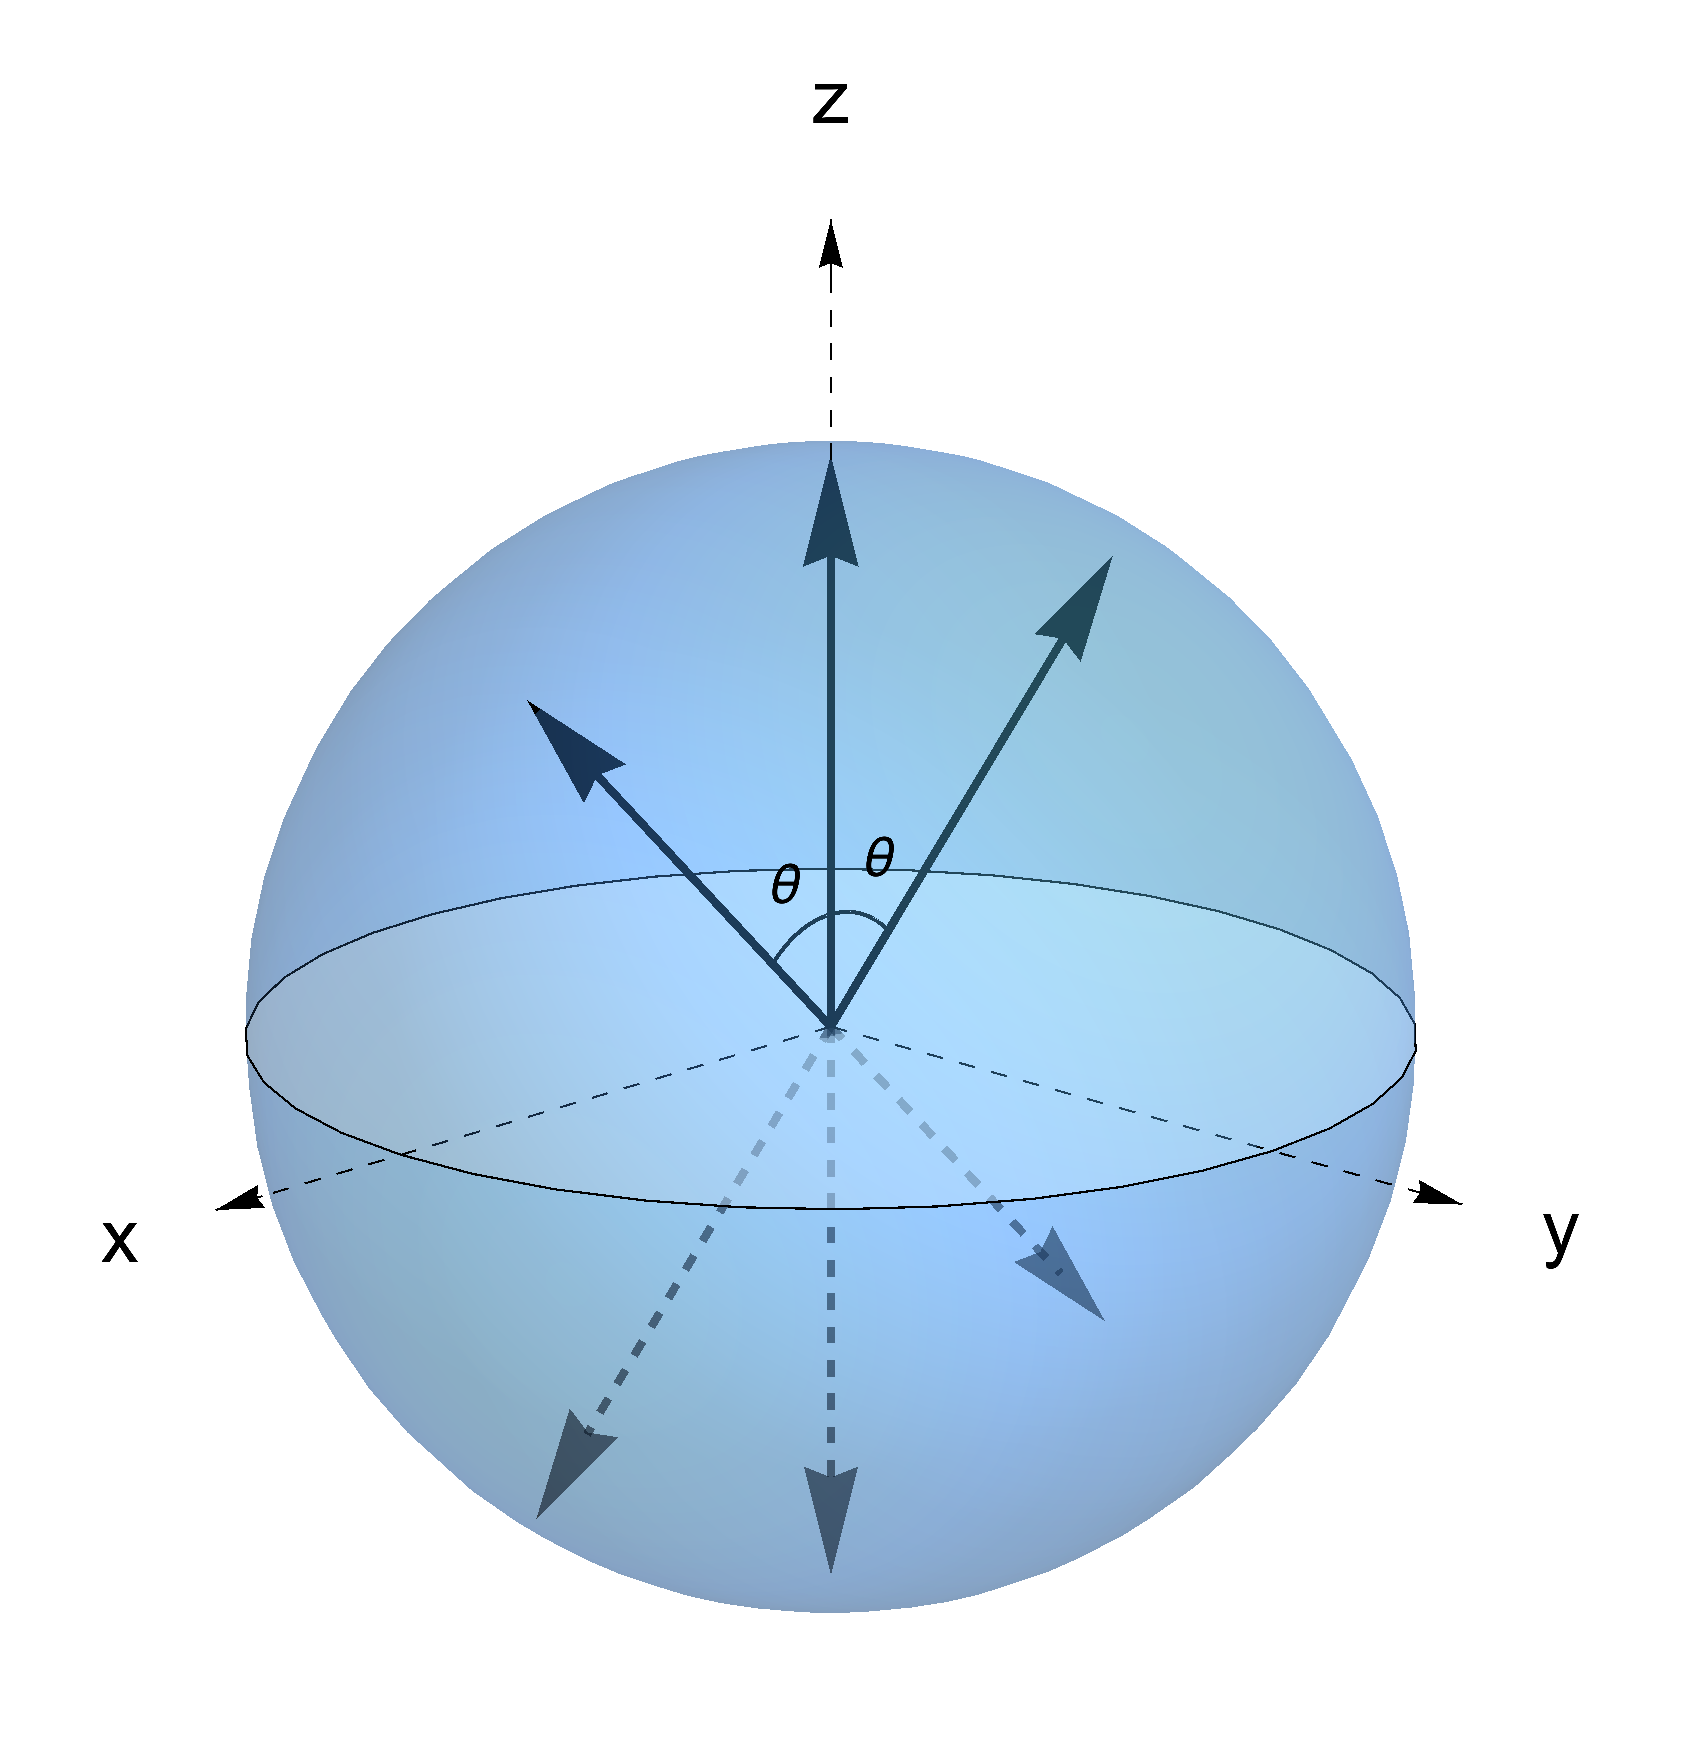
\includegraphics[width=.55\columnwidth]{mirror-symmetric-measurements.png}
            %     \caption{Measurements used to show the existence of classical, non-jointly measurable measurements. The projection on $\mathbf{z}$ and its antipodal effect are fixed, while the two other measurements vary with $0 \leq \theta \leq \pi/2$. In the upper bound, they degenerate in an $\mathbf{x}$ measurement.}
            % \label{fig:mirror-symmetric-measurements}
            % \end{figure}
            % %
            % \begin{figure}
            %     \centering
            %     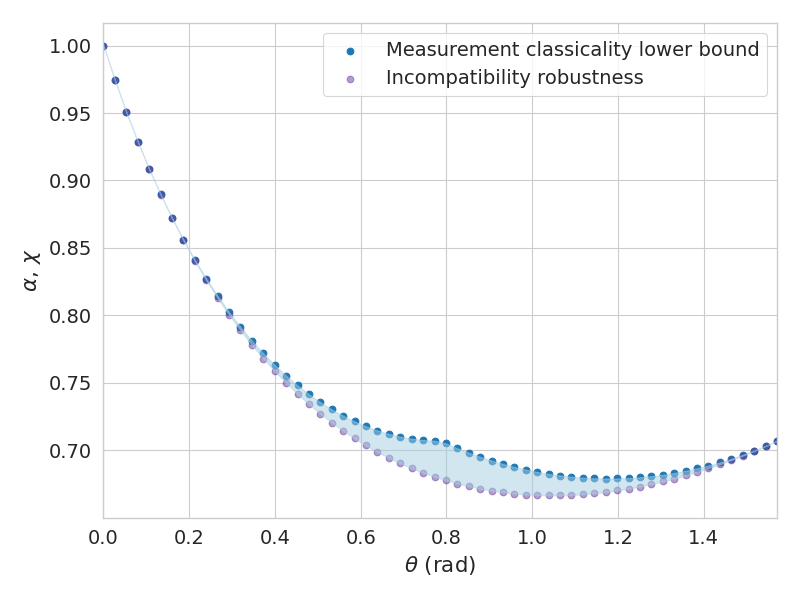
\includegraphics[width=.8\columnwidth]{incompatibility-vs-classicality.png}
            %     \caption{Incompatibility is insufficient for non-classicality in the prepare and measure scenario. For each $\theta$ (see fig. \ref{fig:mirror-symmetric-measurements}), any $\chi$ above the incompatibility robustness curve stands for an incompatible measurement set, and any $\alpha$ below the measurement classicality lower bound represents measurements that certifiedly do not generate non-classical statistics, regardless what preparations they act upon. Thenceforth, the shaded region contains incompatible albeit classical measurements.}
            % \label{fig:incompatibility-vs-classicality}
            % \end{figure}

			\begin{figure*}[t!]
				\newdimen\subfigcapmargin  \subfigcapmargin  =  -3em
				\centering
				%
				\subfigure[]{\label{fig:mirror-symmetric-measurements}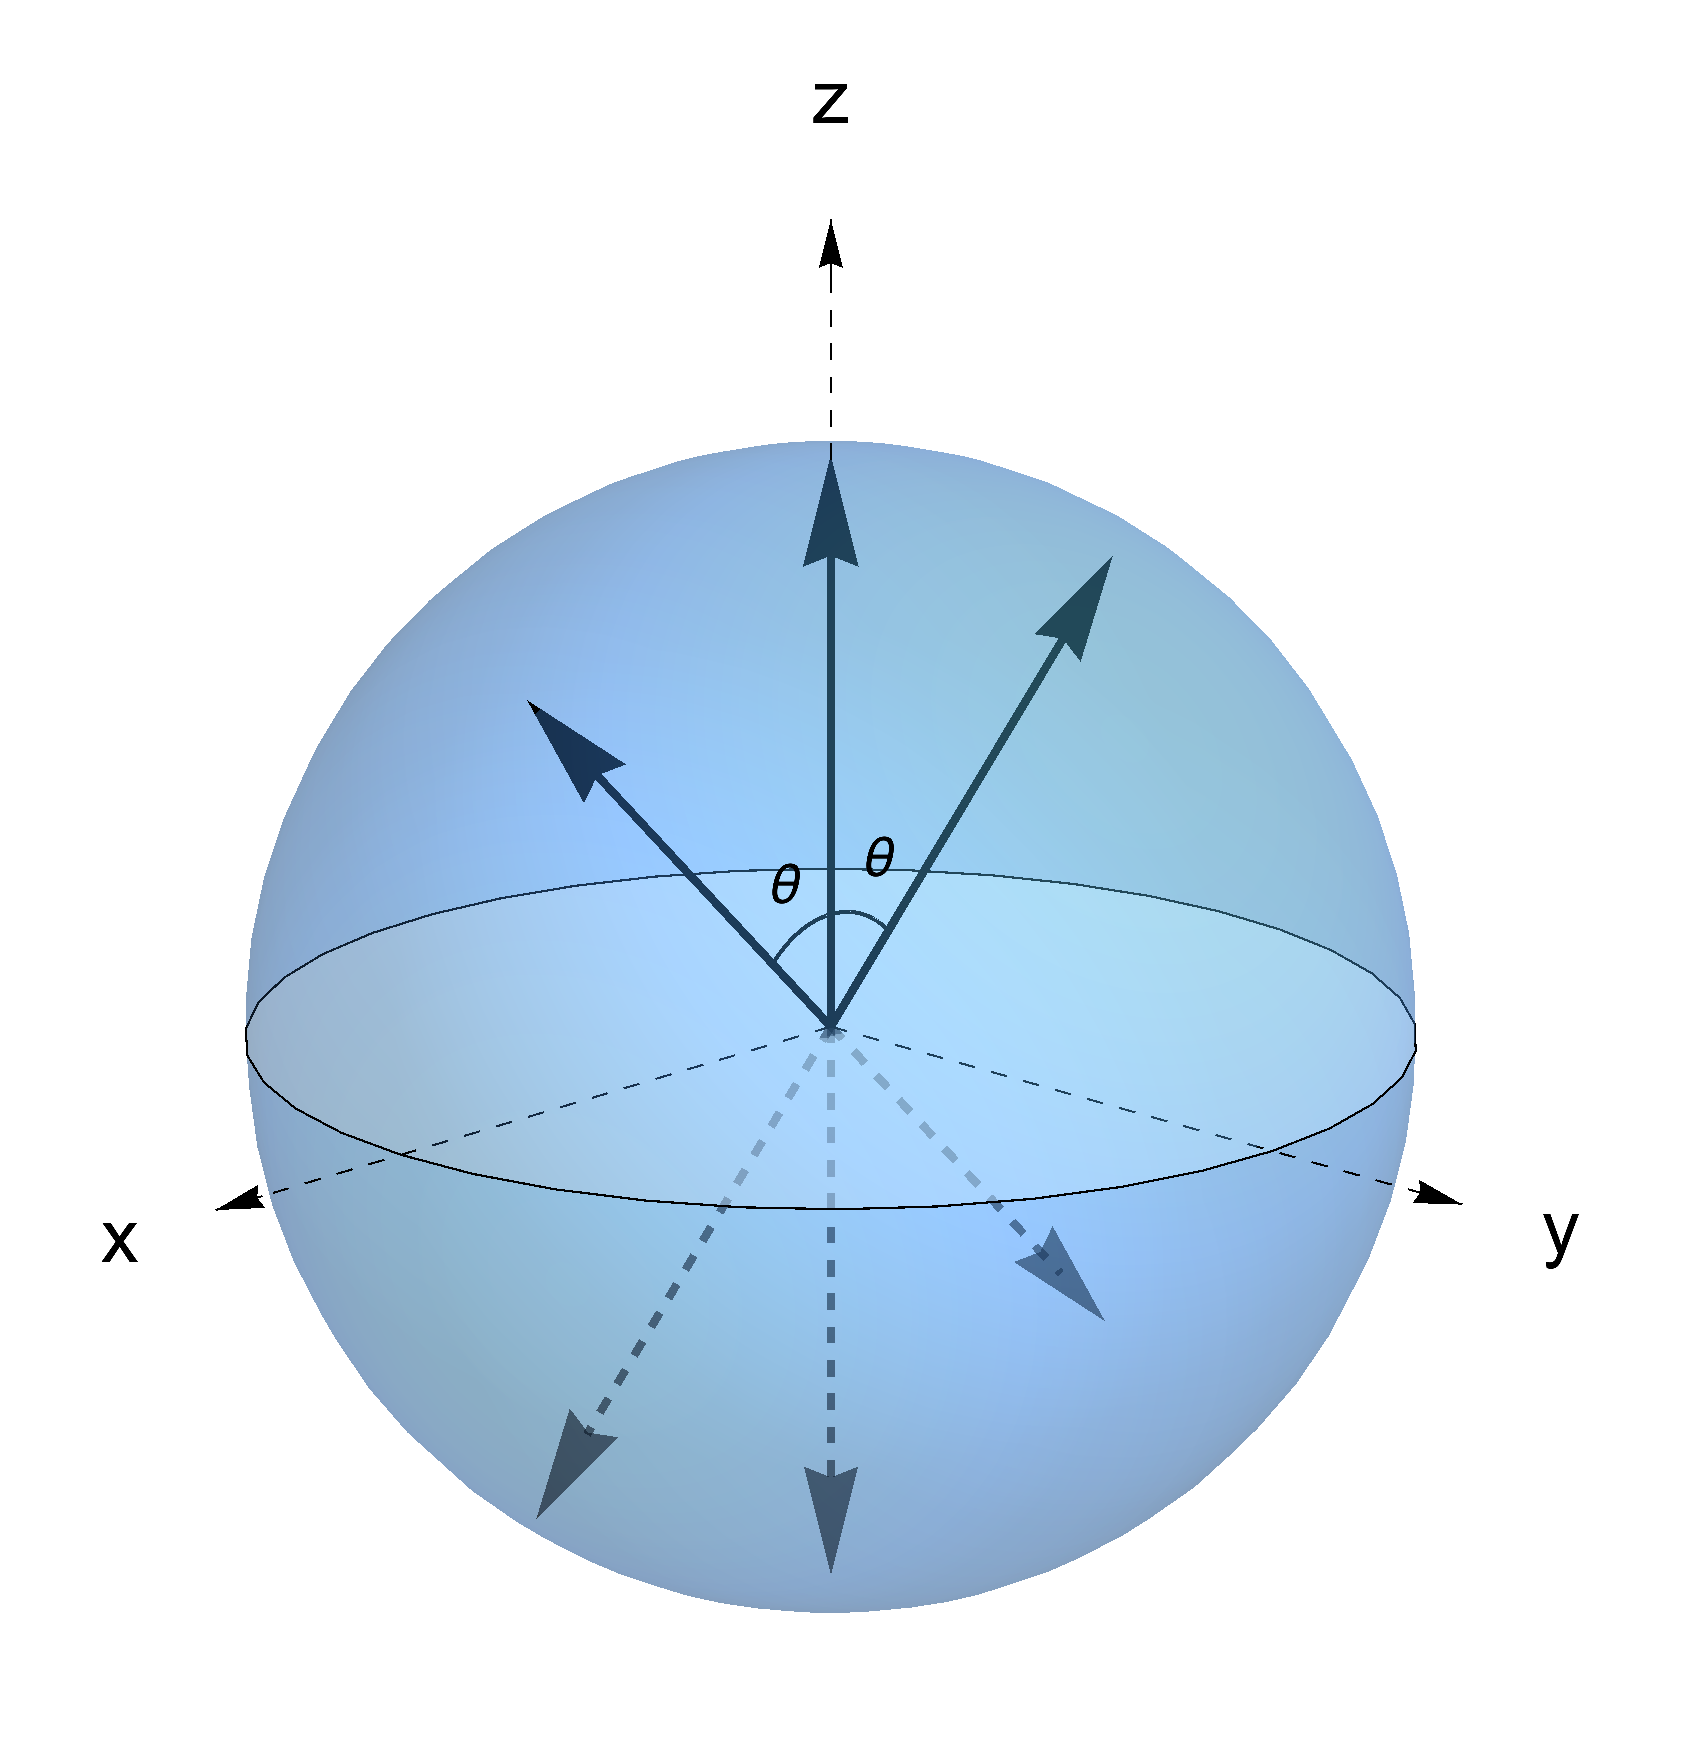
\includegraphics[width=.4\linewidth]{mirror-symmetric-measurements.png}}\hfill
				\subfigure[]{\label{fig:incompatibility-vs-classicality}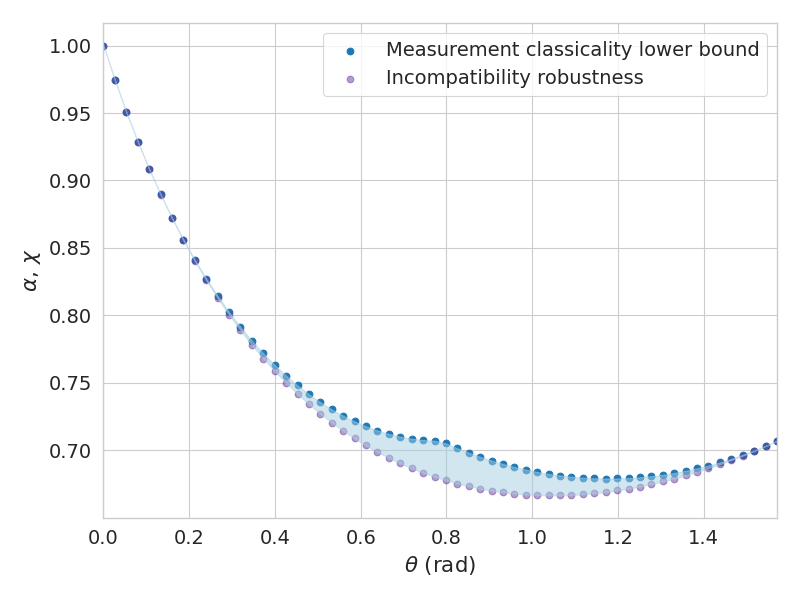
\includegraphics[width=.58\linewidth]{incompatibility-vs-classicality.png}}\hfill
				%
				\caption{Incompatibility is insufficient for non-classicality in the prepare and measure scenario. On the left, parametrized measurements used in the demonstration. The projection on $\mathbf{z}$ and its antipodal effect are fixed, while the two other measurements vary with $0 \leq \theta \leq \pi/2$. In the upper bound, they degenerate in an $\mathbf{x}$ measurement. On the right, program~\eqref{eq:measurement-classicality-projective} was applied. For each $\theta$ (see fig. \ref{fig:mirror-symmetric-measurements}), any $\chi$ above the incompatibility robustness curve stands for an incompatible measurement set, and any $\alpha$ below the measurement classicality lower bound represents measurements that certifiedly do not generate non-classical statistics, regardless what preparations they act upon. Thenceforth, the shaded region contains incompatible albeit classical measurements.}
			\end{figure*}

            Program~\eqref{eq:measurement-classicality-projective} was used to generate the upper curve in the same figure. Twenty-four probe preparations were disposed as the vertices of a rhombicuboctahedron, leading to $\eta \approx 0.86$, and the deterministic strategies were iteratively explored following the algorithm described in appendix \ref{ap:a-computational}. For each $\theta$, the obtained $\alpha$ is a lower bound on the visibility of $\mathcal{M}$ such that a classical model exists for all preparations. Specifically, anything below the classicality curve defines a measurement set which cannot generate nonclassical behaviors. The non-empty region between these two curves certifies there are plenty of incompatible measurements which are classical. Accordingly, non-joint measurability is insufficient for nonclassicality in the prepare-and-measure scenario.


        %%%%%%%%%%%%%%%%%%%%%%%%%%%
        \section{Open questions}

        Albeit the applications discussed in secs. \ref{sec:nonclassicality-activation} and \ref{sec:incompatibility-vs-classicality} rely on the projective measurements case of our criterion, their respective instances for generalized measurements are easily implementable. They do, however, incur in more demanding computational requirements, as the measurement depolarization factor $t$ can be seen as effectively lowering the insphere radius $\eta$. It could nevertheless be interesting to investigate applications of it, as for instance searching for a nonclassicality activation phenomenon valid for all POVMs.

        A second kind of activation phenomenon, emerging by adding more measuremens instead of preparations, has also been observed when the number of preparations is limited \cite{poderini_pamcriteria_2020}. Similarly to sec. \ref{sec:nonclassicality-activation}, the measurement classicality criterion derived in sec. \ref{sec:measurement-classicality} could be used to attempt on finding a more general form of this result, where all preparations are considered.

        Another interesting question is whether POVMs can be used to demonstrate nonclassicality when all PVMs fail to do so. One could approach this in the following manner. Start by selecting classical preparation sets from the results in sec. \ref{sec:nonclassicality-activation} --- which are certifiedly classical for all projective measurements. Then characterize the facets of a $(d=2, B>2, X=3,Y)$ prepare-and-measure polytope. Finally, look for a set of POVMs that, for some of those classical preparation sets, violates any of the obtained facets.

        In view of the method itself, choosing $\Phi$ as the noise model is a natural but not required choice. Different transformations, such as inscribing an ellipsis instead of a depolarized Bloch ball in $\conv{\mathcal{M}}$ (and then applying the corresponding dual map to the preparations) could lead to better computational results, and, potentially, to new insights \cite{fillettaz_algorithmic_2018}.

		The relationship of prepare-and-measure scenarios with random access coding, which was only superficially explored in sec. \ref{sec:racs} and sec. \ref{sec:nonclassicality-activation}, also deserves more exploration. Although the mapping of a RAC to a PM scenario can be trivially done, this is not enough to prove a RACs $\psuc$ is always a facet of the corresponding PM polytope. Believing that, as in the $\rac{2}{2}{1}$, this was always the case, we have further investigated this question. It turns out this is not true. In the general case, a RAC's $\psuc$ must then be some lower dimensional face of prepare-and-measure polytopes. One possible direction is to investigate whether there are subclasses of RACs with this property, of which the $\rac{2}{2}{1}$ is but one example. Another is to explore the meaning of other classes of inequalities defining PM polytopes, and if they represent other instances of information retrieval tasks.

        We believe all these suggestions are worthy of pursuit. Implementations of the programs used in this chapter could be helpful to some of these questions, and are available at a public code repository \cite{classicality_repository}.